\tikzset{
	nfbox/.style={draw,rounded corners,color=uofgsandstone,fill=uofgsandstone!5},
	membox/.style={draw,color=uofgsandstone,fill=uofgsandstone!5},
	idbox/.style={draw,color=uofgpillarbox,fill=uofgpillarbox!5},
	actbox/.style={draw,color=uofgpumpkin,fill=uofgpumpkin!5},
	authflow/.style={color=uofgthistle,thick},
	putflow/.style={color=uofgpillarbox,thick,dash dot},
	readflow/.style={color=uofgcobalt,thick,dash dot},
	zoomflow/.style={color=uofgcobalt!50,thick,dotted},
}

\begin{tikzpicture}
\node (rxq) {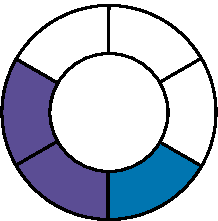
\includegraphics[keepaspectratio,width=3em]{images/ringbuf}};
\node (rxq-l) at ($(rxq) + (0,-0.75)$) {Rx};

\node (txq) at ($(rxq) + (0,-1.5)$) {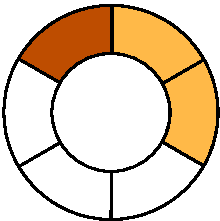
\includegraphics[keepaspectratio,width=3em]{images/ringbuf-alt}};
\node (txq-l) at ($(txq) + (0,-0.75)$) {Tx};

\node (cq) at ($(txq) + (0,-1.5)$) {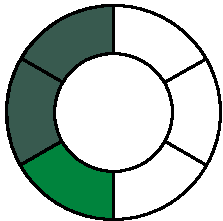
\includegraphics[keepaspectratio,width=3em]{images/ringbuf-alt2}};
\node (cq-l) at ($(cq) + (0,-0.75)$) {Completion};

\node (umem) at ($(rxq) + (3.5,0)$) {
	\begin{tikzpicture}
		\node[rotate=90] (umem-label) at (0,0) {\textsc{Umem}};
		\draw[membox, opacity=0.5] ($(umem-label) + (0.25,0.25)$) rectangle ++(4,0.25);
		\draw[membox] ($(umem-label) + (0.25,0)$) rectangle ++(4,0.25);
		\draw[membox, opacity=0.5] ($(umem-label) + (0.25,-0.25)$) rectangle ++(4,0.25);
		\draw[membox, opacity=0.5] ($(umem-label) + (0.25,-0.5)$) rectangle ++(4,0.25);
		
		\draw[actbox] ($(umem-label) + (0.25,0)$) rectangle ++(1.5,0.25);
		\draw[idbox] ($(umem-label) + (0.25,0)$) rectangle ++(0.75,0.25);
		
		\node[color=uofgpillarbox] at ($(umem-label) + (0.62,0.125)$) {\scriptsize{NF ID}};
		\node[color=uofgpumpkin!50!uofgpillarbox] at ($(umem-label) + (1.38,0.125)$) {$\circledast$};
		\node[color=uofgsandstone] at ($(umem-label) + (3,0.11)$) {\scriptsize{Packet Body}};
	\end{tikzpicture}
};

\node[draw, rectangle, align=left] (b1) at (3.5,-1) {Get packet(s)};
\node[draw, rectangle, align=left] (b2) at ($(b1) + (0,-0.8)$) {\texttt{next\_nf(ID,$\circledast$)}};
\node[draw, rectangle, align=left] (b3) at ($(b2) + (0,-0.8)$) {\texttt{nf\_dylib(pkt,$\triangle$)}};
\node[draw, rectangle, align=left] (b4) at ($(b3) + (0,-0.8)$) {Cleanup};

\node (nfs) at (7,-2.5) {
	\begin{tikzpicture}
		\draw[nfbox, opacity=0.25] (0.2,-0.2) rectangle ++(1,1);
		\draw[nfbox, opacity=0.5] (0.1,-0.1) rectangle ++(1,1);
		\draw[nfbox] (0,0) rectangle ++(1,1);
		
		\node at (0.5,0.4) {\faMicrochip};
		\node at (0.35,0.85) {\scriptsize{\textbf{NF \emph{b}}}};
	\end{tikzpicture}
};

\draw[-,zoomflow] (0.22,-0.18) -- (1.4,0.24);
\draw[-,zoomflow] (0.4,-0.24) -- (1.4,0);

\draw[->, authflow] (b1.east) to[out=-10,in=90] (b2.north east);
\draw[->, authflow] (b2.east) to[out=-10,in=10] node[midway, right] {$\triangle$} (b3.east);
\draw[->, authflow] (b3.south west) to[out=-180,in=180, parabola height=1cm] node[midway, left, sloped, yshift=0.25cm, xshift=0.75cm] {\texttt{Call:} $\triangle'$} (b3.north west);
\draw[->, authflow] (b3.south east) to[out=-30,in=10, parabola height=1cm] (b4.east);

\draw[->, authflow, opacity=0.25] (b4.west) to[out=-180,in=-180, parabola height=-5cm] (b1.west);

\draw[->, readflow] (rxq) to node[midway, below, xshift=-0.4cm] {\footnotesize\texttt{read()}} (b1.west);
\draw[->, readflow] (nfs) to node[midway, below] {\footnotesize\texttt{get($\triangle$)}} (b3.east);

\draw[->, putflow] (b4) to[out=-170, in=-30] node[midway, below] {\footnotesize\texttt{Drop}} (cq);
\draw[->, putflow] ($(b3.west) + (-0.55,0)$) to node[midway, below] {\footnotesize\texttt{Tx}} (txq);
\end{tikzpicture}